\documentclass[11pt]{article}
\usepackage[margin=1in]{geometry}
\usepackage[T1]{fontenc}
\usepackage{lmodern}
\usepackage{booktabs}
\usepackage{amssymb}
\usepackage{enumitem}
\usepackage{listings}
\usepackage{tikz}
\usetikzlibrary{positioning,arrows.meta}
\usepackage[hidelinks]{hyperref}

\setlist{itemsep=2pt,topsep=4pt}
\setlength{\parindent}{0pt}
\setlength{\parskip}{6pt}

\lstset{
  basicstyle=\ttfamily\small,
  keywordstyle=\bfseries,
  commentstyle=\itshape,
  stringstyle=\ttfamily,
  frame=single,
  framesep=4pt,
  breaklines=true,
  columns=fullflexible,
  keepspaces=true,
  showstringspaces=false,
  upquote=true,
}
\lstdefinelanguage{json}{basicstyle=\ttfamily\small}

\tikzset{
  box/.style={draw, thick, minimum height=9mm, minimum width=22mm, align=center, font=\small},
  dbox/.style={box, dashed},
  arr/.style={-{Stealth[length=2.5mm]}, thick},
}

\title{\textbf{CLAWS Onboarding: EVA Voice Intent Model}}
\author{CLAWS Voice Assistant Team}
\date{Fall 2026}

\begin{document}
\maketitle

\textbf{Goal:} write training sentences for 35 EVA intents, fine-tune a small
model, classify sentences it has never seen. Text in, intent out is required.
Voice (Whisper + TTS) is a stretch goal. Shared code is in
\texttt{code/}; your work goes in your own folder.

\section{Where this fits}

\begin{center}
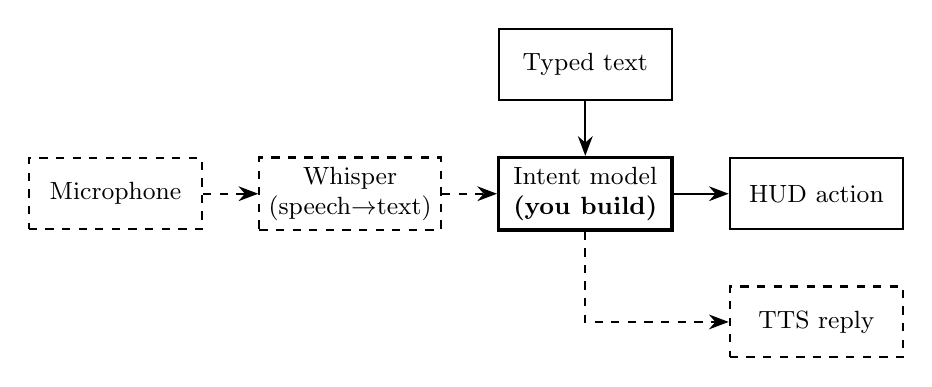
\begin{tikzpicture}[node distance=7mm]
  \node[dbox] (mic) {Microphone};
  \node[dbox, right=of mic] (stt) {Whisper\\(speech$\to$text)};
  \node[box, right=of stt, very thick] (model) {Intent model\\\textbf{(you build)}};
  \node[box, right=of model] (hud) {HUD action};
  \node[dbox, below=of hud] (tts) {TTS reply};
  \node[box, above=of model] (text) {Typed text};
  \draw[arr, dashed] (mic) -- (stt);
  \draw[arr, dashed] (stt) -- (model);
  \draw[arr] (text) -- (model);
  \draw[arr] (model) -- (hud);
  \draw[arr, dashed] (model) |- (tts);
\end{tikzpicture}
\end{center}

Solid = required. Dashed = stretch. The model picks an intent (plus a name for
five intents). The HUD reads the actual value from telemetry.

\newpage
\section{The intents}

Labels are \textbf{case-sensitive}. Copy them exactly. Also in
\texttt{code/intents.json}.

\begin{center}
\small
\begin{tabular}{@{}llc@{}}
\toprule
Intent & Meaning & Name \\
\midrule
\texttt{get\_oxy\_pri\_storage} & Primary oxygen storage \% & \\
\texttt{get\_oxy\_sec\_storage} & Secondary oxygen storage \% & \\
\texttt{get\_oxy\_pri\_pressure} & Primary oxygen tank pressure & \\
\texttt{get\_oxy\_sec\_pressure} & Secondary oxygen tank pressure & \\
\texttt{get\_suit\_pressure\_oxy} & Suit O$_2$ partial pressure & \\
\texttt{get\_suit\_pressure\_co2} & Suit CO$_2$ partial pressure & \\
\texttt{get\_suit\_pressure\_other} & Suit trace gas pressure & \\
\texttt{get\_suit\_pressure\_total} & Total suit pressure & \\
\texttt{get\_helmet\_pressure\_co2} & Helmet CO$_2$ pressure & \\
\texttt{get\_fan\_pri\_rpm} & Primary fan speed (RPM) & \\
\texttt{get\_fan\_sec\_rpm} & Secondary fan speed (RPM) & \\
\texttt{get\_scrubber\_a\_co2\_storage} & Scrubber A CO$_2$ storage & \\
\texttt{get\_scrubber\_b\_co2\_storage} & Scrubber B CO$_2$ storage & \\
\texttt{get\_temperature} & Suit internal temperature & \\
\texttt{get\_coolant\_storage} & Coolant storage \% & \\
\texttt{get\_coolant\_gas\_pressure} & Coolant gas loop pressure & \\
\texttt{get\_coolant\_liquid\_pressure} & Coolant liquid loop pressure & \\
\texttt{get\_heart\_rate} & Astronaut heart rate & \\
\texttt{get\_oxy\_consumption} & Oxygen consumption rate & \\
\texttt{get\_co2\_production} & CO$_2$ production rate & \\
\texttt{get\_eva\_elapsed\_time} & Elapsed mission time & \\
\texttt{get\_primary\_battery\_level} & Primary battery \% & \\
\texttt{get\_secondary\_battery\_level} & Secondary battery \% & \\
\texttt{get\_warnings} & Active warnings and alerts & \\
\midrule
\texttt{open\_menu\_vitals} & Open vitals panel & \\
\texttt{open\_menu\_navigation} & Open navigation / map panel & \\
\texttt{open\_menu\_tasks} & Open tasks / checklist panel & \\
\texttt{open\_menu\_uia} & Open UIA airlock panel & \\
\texttt{close\_menu} & Close the active panel & \\
\midrule
\texttt{Get\_coordinates} & Coordinates of a named target & $\checkmark$ \\
\texttt{Set\_navigation\_target} & Navigate to a named place & $\checkmark$ \\
\texttt{reroute\_navigation} & Compute a new route & \\
\texttt{Add\_waypoint} & Add a named waypoint & $\checkmark$ \\
\texttt{Delete\_waypoint} & Delete a named waypoint & $\checkmark$ \\
\texttt{Complete\_task} & Mark a named task complete & $\checkmark$ \\
\bottomrule
\end{tabular}
\end{center}

\newpage
\section{Setup}

Any laptop works (CPU is fine; MPS/CUDA used if present). Python 3.9+.
Your folder is already made:

\begin{center}
\begin{tabular}{@{}ll@{}}
\toprule
Member & Folder \\
\midrule
Aaron  & \texttt{submissions/aaron/} \\
Evan   & \texttt{submissions/evan/} \\
Raiana & \texttt{submissions/raiana/} \\
Sam    & \texttt{submissions/sam/} \\
Utsav  & \texttt{submissions/utsav/} \\
Vivian & \texttt{submissions/vivian/} \\
\bottomrule
\end{tabular}
\end{center}

\begin{lstlisting}[language=bash]
git clone https://github.com/CLAWS-UMICH/AI-Onboarding-2026.git && cd AI-Onboarding-2026
git checkout -b onboarding/<your-name>
python3 -m venv .venv && source .venv/bin/activate
pip install torch transformers sentence-transformers scikit-learn
cd submissions/<your-name>        # run everything from here
\end{lstlisting}

Each folder has an empty \texttt{data/train.jsonl}, an empty \texttt{runs/},
and a \texttt{notes.md} template. Run scripts from your folder as
\texttt{python ../../code/<script>.py}; data and results land in your folder.
Don't copy the code into your folder.

\newpage
\section{Write the training data}

The model is only as good as your sentences. One file,
\texttt{data/train.jsonl}, one JSON object per line, exactly one intent each
(same format as \texttt{EVA/data/}):

\begin{lstlisting}[language=json]
{"text": "what's my primary oxygen at", "intents": ["get_oxy_pri_storage"]}
{"text": "O2 secondary tank pressure?", "intents": ["get_oxy_sec_pressure"]}
{"text": "uh how hot is it in the suit", "intents": ["get_temperature"]}
{"text": "pull up the map", "intents": ["open_menu_navigation"]}
{"text": "drop a waypoint called Crater Rim", "intents": ["Add_waypoint"]}
\end{lstlisting}

\textbf{Rules}
\begin{itemize}
  \item \textbf{30+ per intent} (50 ideal). Write them yourself; LLM ideas OK if you check every line.
  \item Mix questions, commands and clipped phrases (``fan RPM?''). 2 to 20 words.
  \item Vary words: oxygen/O2/ox, battery/charge/power, menu/panel/screen.
  \item Sound like speech: ``uh'', ``please'', lowercase, no punctuation.
  \item Always say which one: primary/secondary, A/B, gas/liquid.
  \item Vary names in the five name intents. No near-duplicates.
\end{itemize}

\lstinputlisting[language=Python, caption={\texttt{validate.py}}]{code/validate.py}

\begin{lstlisting}[language=bash]
python ../../code/validate.py data/train.jsonl   # fix until "0 problems"
\end{lstlisting}

\newpage
\section{Build the model}

\textbf{Step 0: baseline.} Frozen sentence embeddings + logistic regression.
This is the number to beat.

\lstinputlisting[language=Python, caption={\texttt{baseline.py}}]{code/baseline.py}

\begin{lstlisting}[language=bash]
python ../../code/baseline.py > baseline.txt
\end{lstlisting}

\textbf{Step 1: fine-tune.} MiniLM (22M params) + mean pooling + one linear
layer, same as the club model in \texttt{EVA/Models/singleintentmodel/}.

\begin{center}
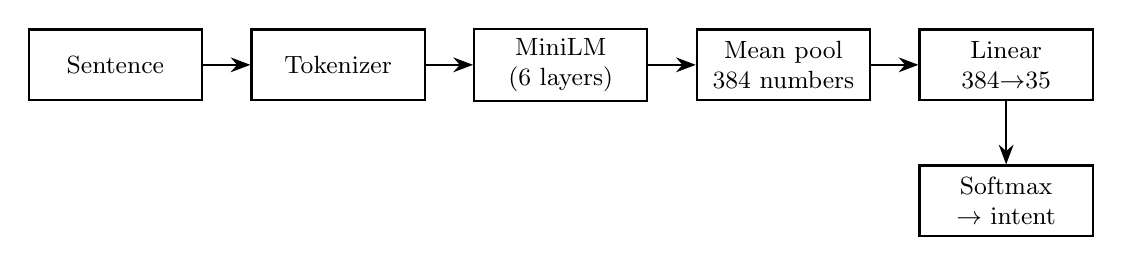
\begin{tikzpicture}[node distance=6mm]
  \node[box] (in) {Sentence};
  \node[box, right=of in] (tok) {Tokenizer};
  \node[box, right=of tok] (enc) {MiniLM\\(6 layers)};
  \node[box, right=of enc] (pool) {Mean pool\\384 numbers};
  \node[box, right=of pool] (head) {Linear\\384$\to$35};
  \node[box, below=8mm of head] (out) {Softmax\\$\to$ intent};
  \draw[arr] (in) -- (tok);
  \draw[arr] (tok) -- (enc);
  \draw[arr] (enc) -- (pool);
  \draw[arr] (pool) -- (head);
  \draw[arr] (head) -- (out);
\end{tikzpicture}
\end{center}

\lstinputlisting[language=Python, caption={\texttt{model.py}}]{code/model.py}

\texttt{train.py} holds out 15\%, trains 10 epochs, prints accuracy each epoch,
then lists every miss. Expect $>$0.95 and a win over the baseline; if not, fix
your data.

\lstinputlisting[language=Python, caption={\texttt{train.py}}]{code/train.py}

\begin{lstlisting}[language=bash]
python ../../code/train.py
\end{lstlisting}

\newpage
\section{Evaluate and predict}

\lstinputlisting[language=Python, caption={\texttt{predict.py}}]{code/predict.py}

\begin{lstlisting}[language=bash]
python ../../code/predict.py "add a waypoint named Olympus Ridge"
{"text": "add a waypoint named Olympus Ridge", "selected_intent": "Add_waypoint",
 "confidence": 0.969, "slot": "Olympus Ridge"}
\end{lstlisting}

\textbf{Held-out accuracy is not the real test.} Write 10+ new sentences
(ideally a friend writes some) and see what breaks. Common confusions:
primary/secondary, scrubber A/B, coolant gas/liquid,
\texttt{open\_menu\_navigation}/\texttt{reroute\_navigation}, and the
coordinate/target/waypoint intents. Fix confusions with better data, not code.

\textbf{Names:} \texttt{extract\_slot} takes the text after the last trigger
word. It's naive (``mark task soil sample complete'' $\to$ \texttt{soil sample
complete}). Improving it is a bonus.

\newpage
\section{Stretch: make it talk}

\begin{lstlisting}[language=bash]
pip install faster-whisper sounddevice pyttsx3
python ../../code/voice.py
\end{lstlisting}

\lstinputlisting[language=Python, caption={\texttt{voice.py}}]{code/voice.py}

Next steps: \texttt{small.en} Whisper, speak the real value back, push-to-talk.

\newpage
\section{What to hand in}

\textbf{One big PR.} Commit as often as you like on your branch, but open a
single PR when everything below is done. No partial PRs. Only touch your own
folder, so the six PRs never conflict.

\begin{itemize}[label=$\square$]
  \item \texttt{data/train.jsonl} (0 problems in \texttt{validate.py})
  \item \texttt{runs/metrics.json}, \texttt{runs/label2id.json}
  \item \texttt{baseline.txt} (output of \texttt{baseline.py})
  \item \texttt{notes.md}: filled in (results, 10+ unseen sentences, what failed)
  \item \textbf{Not} \texttt{runs/model.pt} (\texttt{.gitignore} skips it)
\end{itemize}

Stuck for over an hour? Ask in the channel.

\end{document}
